\documentclass{beamer}
\usetheme{}
\usecolortheme{dolphin}           
\useinnertheme{circles}
\setbeamertemplate{itemize items}[default]
\setbeamertemplate{enumerate items}[default]
\usepackage[T1]{fontenc}
\usepackage[utf8]{inputenc}
\usepackage{lmodern}
\usepackage{amsmath}
\usepackage{booktabs} 
\usepackage{graphicx}        
\usepackage{array}
\usepackage{color}
\makeatletter
\def\zapcolorreset{\let\reset@color\relax\ignorespaces}
\def\colorrows#1{\noalign{\aftergroup\zapcolorreset#1}\ignorespaces}
\makeatother
\graphicspath{{/home/swl/Dropbox/ucd/advanced_macro/figures/}} 
\setbeamertemplate{navigation symbols}{}

%--------------------------------------
\title{Identification in macroeconomics}
\author{School of Economics, University College Dublin}
\date{Spring 2018}
\begin{document}

%--------------------------------------
\begin{frame}
 \titlepage
\end{frame}
%--------------------------------------

%--------------------------------------
\begin{frame} 
  Some of the main questions in macroeconomics are
  \medskip
  \begin{enumerate}
    \item What causes business cycle fluctuations?
    \item How does monetary or fiscal policy influence the economy?
    \medskip
    \item Why do some countries grow faster than others?
  \end{enumerate}  
\end{frame}
%--------------------------------------

%--------------------------------------
\begin{frame}
  The answers to these questions are often   
  \begin{enumerate}
    \item Unknown
    \item Difficult to find
  \end{enumerate}
\end{frame}
%--------------------------------------

%--------------------------------------
\begin{frame}
  A major complication in finding answers is \textbf{identification}
  \begin{itemize}
    \item As in any empirical field
  \end{itemize}
  \medskip
  Identification means whether or not the unknown parameter value can be deduced from the observed data  
  \begin{itemize}
    \item Consistent estimators may exist under number of assumptions, e.g. central limit theorem
  \end{itemize}
\end{frame}
%--------------------------------------

%--------------------------------------
\begin{frame}
  Why do we need an identified model?  
  \begin{itemize}
    \item Necessary condition for the existence of consistent estimators
    \item i.e. when sample size increases, the estimator will converge, probabilistically, to parameter's unknown value
  \end{itemize}  
\end{frame}
%--------------------------------------

%--------------------------------------
\begin{frame}
 For a general definition of identification, let $P$ be the true distribution of observed data $X$ which can be modeled by
 \begin{align}
   \mathbf{P} = \{P_{\theta}: \theta \in \Theta  \}
 \end{align}
 \medskip
 Assuming that 
 \begin{align}
   P \in \mathbf{P} = \{P_{\theta}: \theta \in \Theta  \}
 \end{align}
 or that there is a correctly specified model with parameters $\theta \in \Theta$ such that $P \in \mathbf{P}$.
 Of course we are interested in $\theta$.  
\end{frame}
%--------------------------------------

%--------------------------------------
\begin{frame}
  Suppose that we know for a fact that 
  \begin{align}
    P \in \mathbf{P}
  \end{align}
  \medskip
  This means that there is  
  \begin{align}
    \theta \in \Theta
  \end{align}
  for 
  \begin{align}
    P_{\theta} \in \mathbf{P}
  \end{align}
\end{frame}
%--------------------------------------


%--------------------------------------
\begin{frame}
 One problem however is that we cannot distinguish 
 \begin{align}
   \theta \in \Theta
 \end{align}
 from
 \begin{align}
   \theta^* \in \Theta
 \end{align}
 \medskip
 i.e. from our knowledge about $P$ we can only say that 
  \begin{align}
    \theta \in \Theta_0(P)= \{\theta \in \Theta: P_{\theta} = P\}
  \end{align}
\end{frame}
%--------------------------------------

%--------------------------------------
\begin{frame}
 Given $\theta \in \Theta_0(P)$, $\Theta_0(P)$ is the identified set    
  \begin{itemize}
    \item So $\theta$ is identified if $\Theta_0 (P)$ is a singleton for all $P \in \mathbf{P}$
  \end{itemize} 
  \medskip
  $\mathbf{P}$ should be interpreted as a structural model for the distribution of observed data $X$.
\end{frame}
%--------------------------------------

%--------------------------------------
\begin{frame}
  Two remaining questions
  \begin{enumerate}
    \item Why bother with a structural model?
    \item How can a model be identified?
  \end{enumerate}
\end{frame}
%--------------------------------------

%--------------------------------------
\begin{frame}
 From $P$ we can calculate all kinds of interesting statistics
 \begin{itemize}
   \item Predictors, conditional probabilities, etc.
 \end{itemize}
 \medskip
 Although these statistics provide useful insights about the data, it tells us little about the mechanisms generating the data
 \begin{itemize}
   \item Hence the need for a structural model
 \end{itemize}
 \medskip
 In the identified model the structure of the data $\mathbf{P}$ is given by unknown value $\theta \in \Theta$
 \begin{itemize}
   \item A central question is what we can learn from $\theta$, under certain conditions, from observed distribution $P$?
 \end{itemize}
\end{frame}
%--------------------------------------

%--------------------------------------
\begin{frame}
 So how can a model be identified?
 This can be achieved through
 \begin{enumerate}
    \item Variation
    \item 'Natural experiments'
  \end{enumerate}
\end{frame}
%--------------------------------------

%--------------------------------------
\begin{frame}
 Let's consider a practical example: Fed interest rates
 \begin{itemize}
   \item In 2008 the Fed lowered the rates in a reaction to the financial crisis (later Great Recession)
   \item Lowering interest rates should encourage spending; stimulate economic activity
 \end{itemize}
 \medskip
 Interest rate change are a source of variation in monetary policy: can be used in a model  
\end{frame}
%--------------------------------------

%--------------------------------------
\begin{frame}
  \begin{figure}
    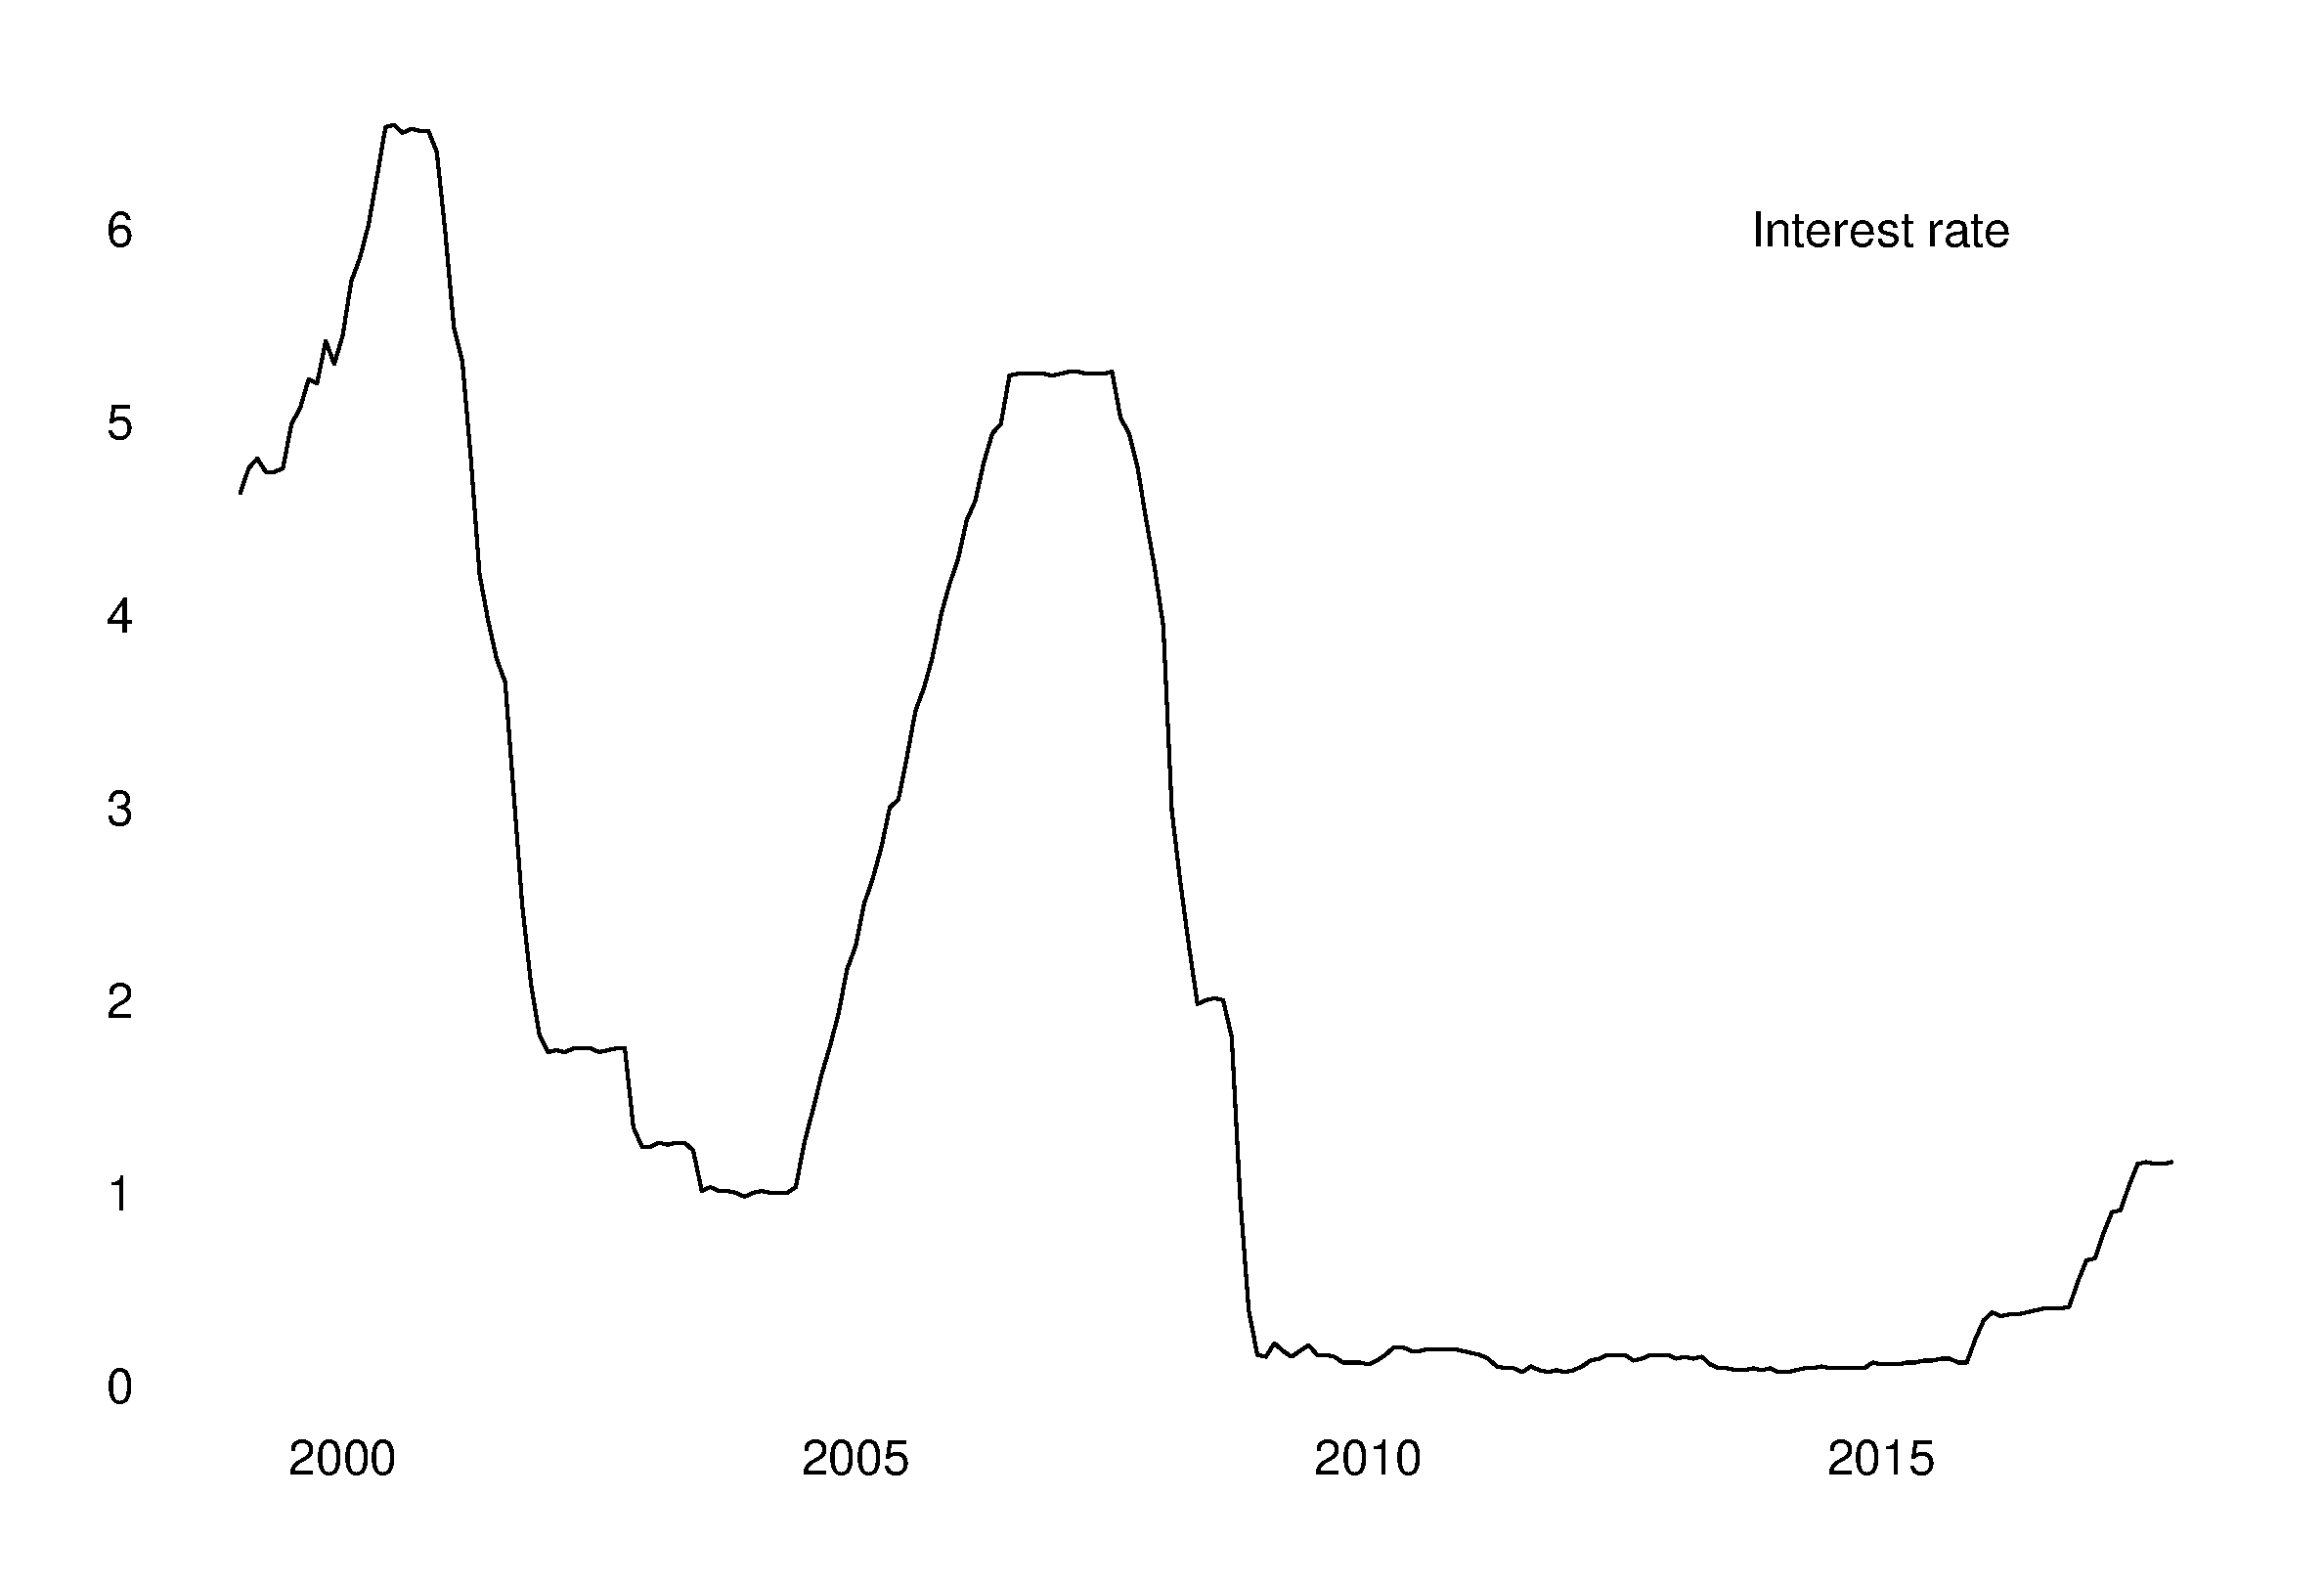
\includegraphics[scale=.3]{effective_rate.eps}
  \end{figure}
\end{frame}
%--------------------------------------

%--------------------------------------
\begin{frame}
  Estimate effect of interest rate on economic output using following model 
  \begin{align}
    \Delta GDP_t = \alpha + \beta \Delta i_t + \epsilon_t
  \end{align}
  \medskip
  Fit model to data using OLS; possible estimate $\beta > 0$
\end{frame}
%--------------------------------------

%--------------------------------------
\begin{frame}
  \begin{figure}
    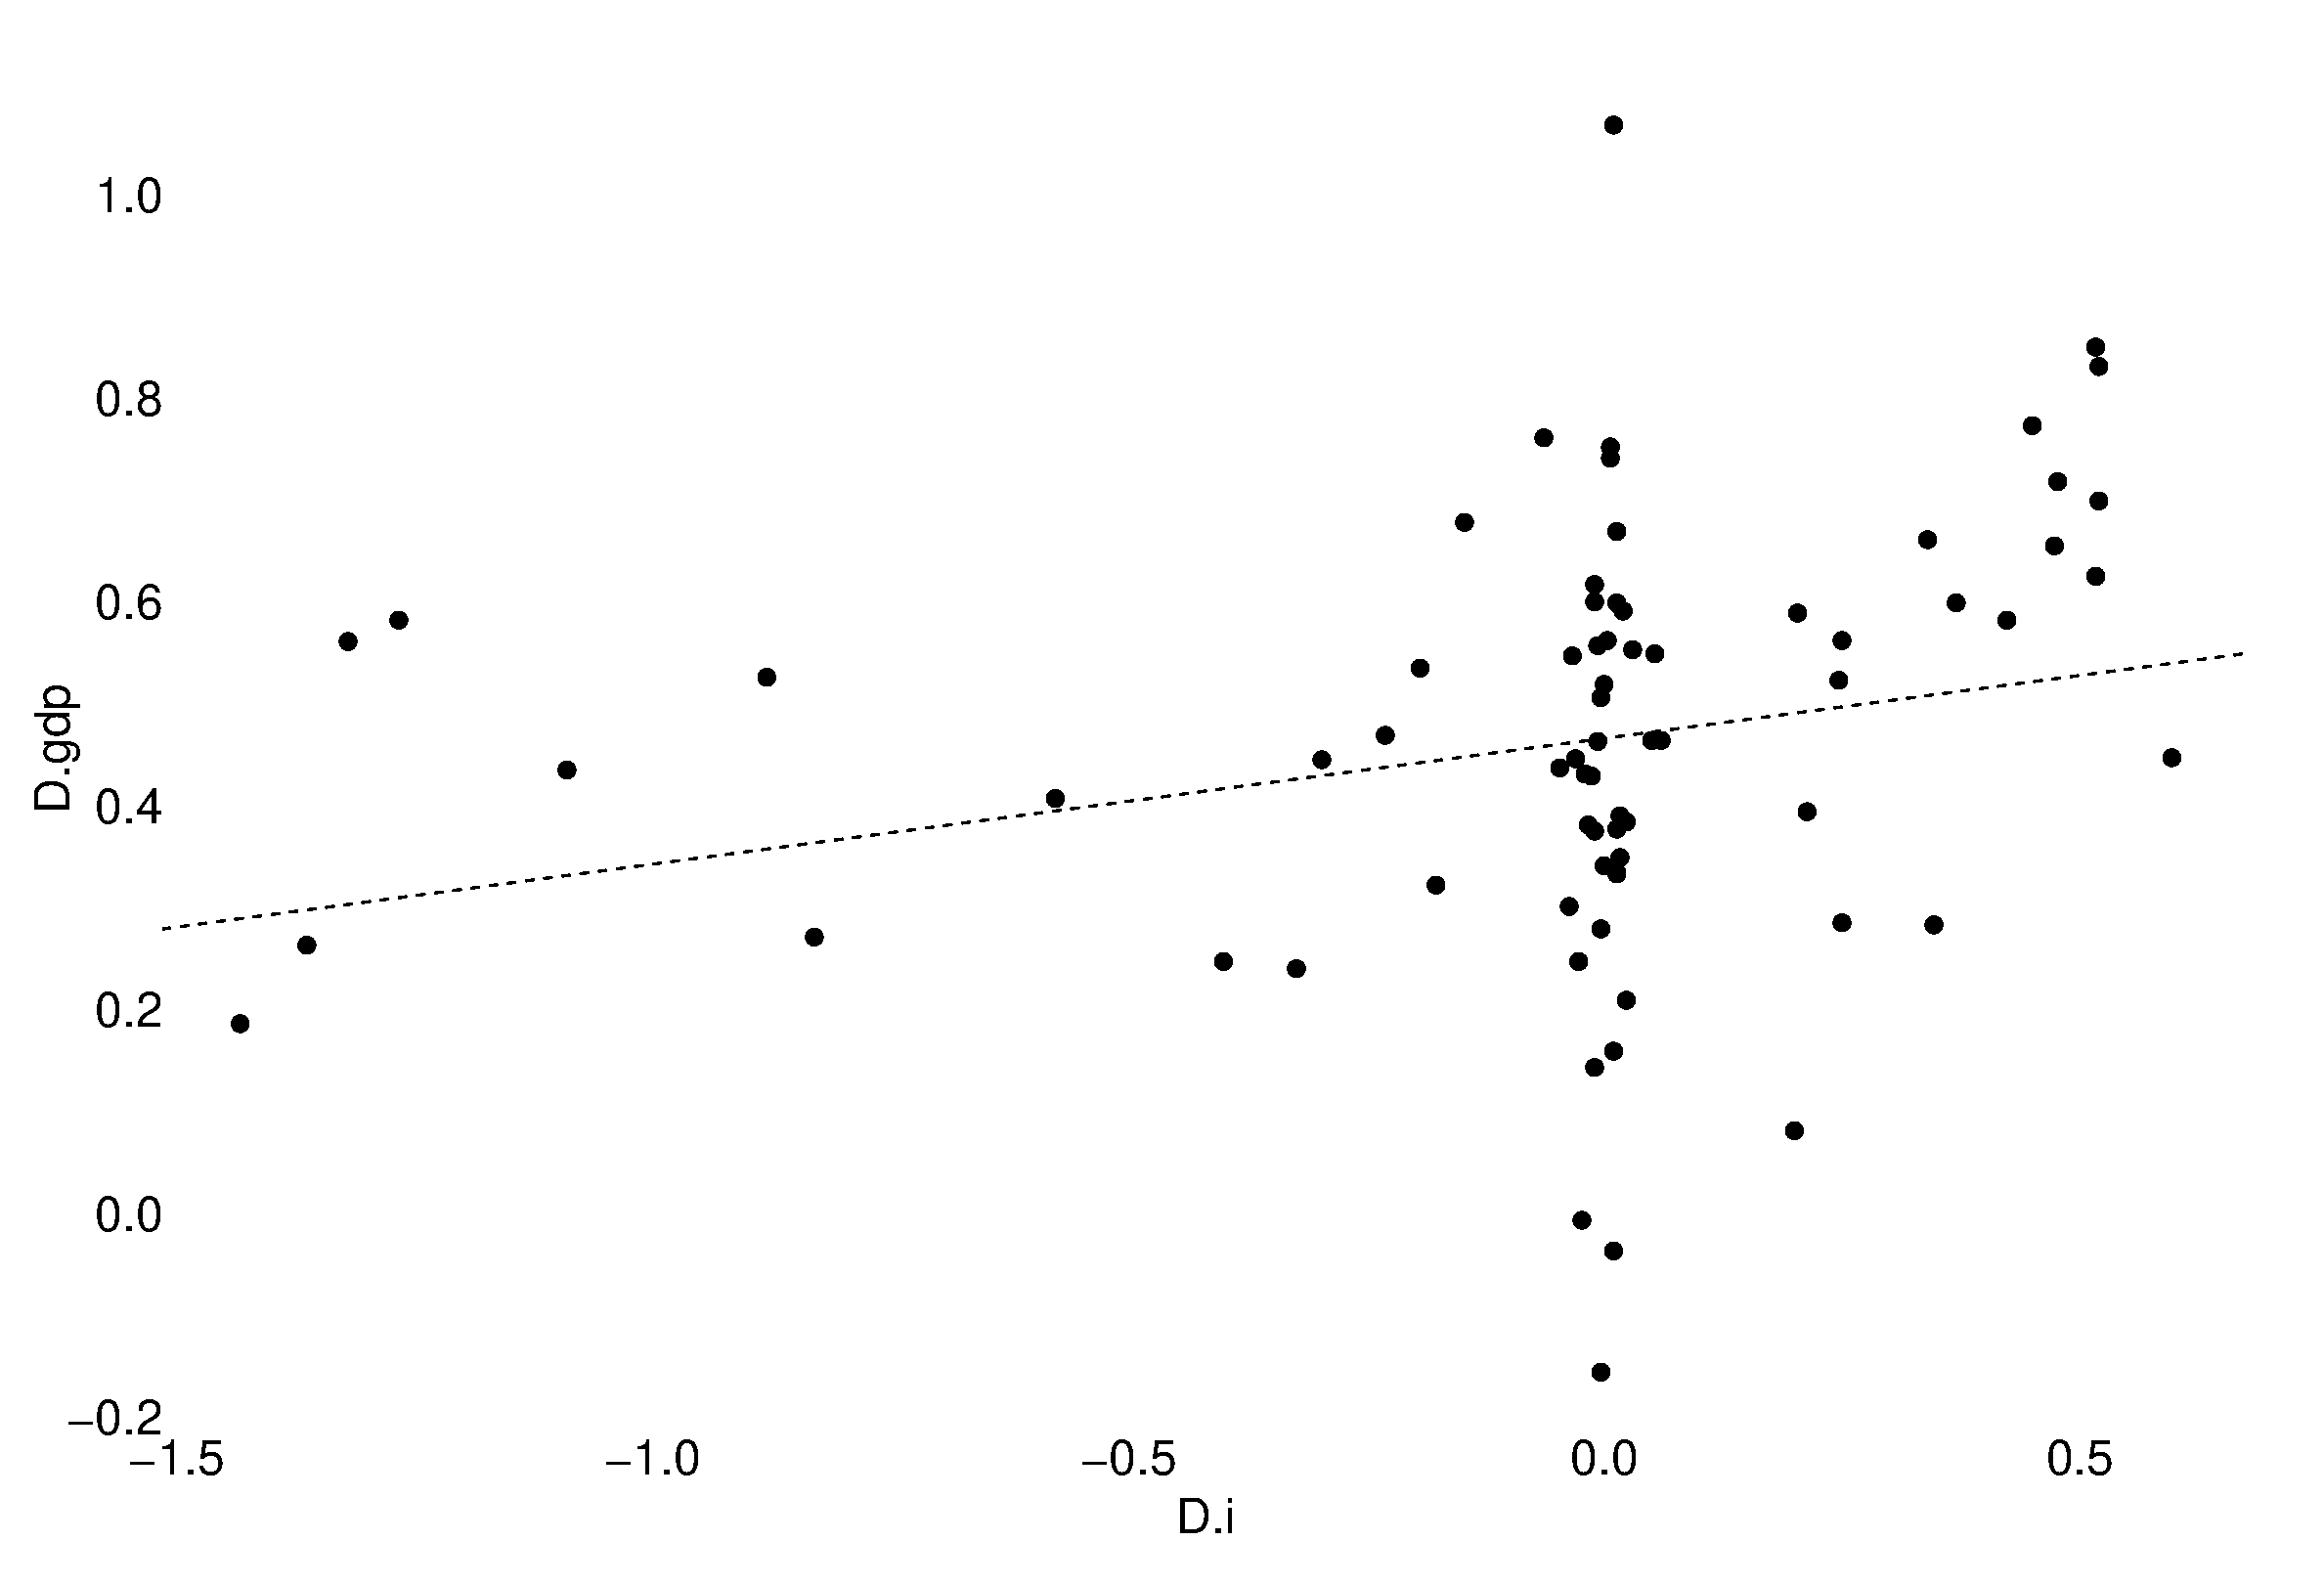
\includegraphics[scale=.3]{lm.eps}
  \end{figure}
\end{frame}
%--------------------------------------

%--------------------------------------
\begin{frame}
 Based on regression results we could conclude that reduction in interest rate correlates/causes decrease in output
 \begin{itemize}
   \item i.e. lowering the interest rate will harm the economy
 \end{itemize}
 \medskip
 Sticking to evidence-based policy, the implication would be to increase the interest rate in order to stimulate economic activity.
\end{frame}
%--------------------------------------

%--------------------------------------
\begin{frame}
  Naturally the Fed does not change interest rates randomly
  \begin{itemize}
    \item They change due to some factor(s) affecting the economy
    \item Around 2008 think of falling house prices and their effect on bank balance sheets
  \end{itemize}
  \medskip
  This means that interest rates are endogenous and that other factors confound the effect of change in monetary policy
  \begin{itemize}
    \item i.e. the regression does not capture the \textbf{isolated} effect of the interest rate.
  \end{itemize}
\end{frame}
%--------------------------------------

%--------------------------------------
\begin{frame}
  Dynamics therefore play an important role in macroeconomic research and this entails two important challenges  
  \begin{enumerate}
    \item Difficult to identify exogenous variation in macroeconomic policy
    \item Natural experiments that can be identified are rarely those required to answer questions we're interested in. 
  \end{enumerate}
  \medskip
  This results into an external validity problem.  
\end{frame}
%--------------------------------------

%--------------------------------------
\begin{frame}
  Some other important issues include
  \medskip
  \begin{enumerate}
   \item Dynamic nature of monetary and fiscal policy make it high dimensional; can have effect on both short and long run
   \item Effects of fiscal shocks depends on monetary policy (constrained by zero lower bound) and tax policy response
   \item Effect of policy depends on the economy
   \item Degree to which a policy is a surprise affects when and how strongly an economy reacts  
 \end{enumerate}
 \medskip
 Therefore, macroeconomic research tends to be structural in nature  
 \begin{itemize}
   \item Different from other empirical economic research which seeks to identify causal effects
 \end{itemize} 
\end{frame}
%--------------------------------------

%--------------------------------------
\begin{frame}
  Applied macroeconomics heavily uses statistical methods and therefore relies on the use of \textbf{moments}  
  \begin{itemize}
    \item Moments characterise the statistical distribution and are most commonly taken around the mean
    \item e.g. mean, variance, etc. 
  \end{itemize}
  \medskip
  We can distinguish between \textbf{identified} and \textbf{unidentified} moments  
  \begin{enumerate}
    \item Unidentified: Simple statistics such as means, variances, and correlations
    \item Identified: Statistics derived from empirical strategies or causal effect estimates 
  \end{enumerate}
\end{frame}
%--------------------------------------

%--------------------------------------
\begin{frame}
 Identified moments are designed to help uncover causal effects (micro) or responses to structural shocks (macro).
 \medskip
 \begin{enumerate}
   \item Micro moments are constructed using microeconomic data on behaviour of individuals and firms
   \item Macro moments use aggregated data to identify equilibrium outcomes; informative about what type of world we live in 
  \end{enumerate} 
  \medskip
  Important to know is whether these moments actually correspond to structural parameters.
\end{frame}
%--------------------------------------

%--------------------------------------
\begin{frame}
  In some cases moment do correspond to structural parameters
  \begin{itemize}
    \item e.g. labour supply elasticity in labour economics
  \end{itemize}
  \medskip
  In other cases they don't
  \begin{itemize}
    \item e.g. marginal propensity to consumer (following transitory fiscal rebate); estimate of regional fiscal multiplier
  \end{itemize}
  \medskip
  When an identified moment does not correspond to a structural parameter, a theoretical framework is needed to go from identified moment to macroeconomic question of interest.
\end{frame}
%--------------------------------------

%--------------------------------------
\begin{frame}
 Finally we have to consider data and the unit-of-analysis; in general a model can be identified at 
 \medskip 
  \begin{enumerate}
    \item Aggregate level; focusing on single country
    \item Cross-sectional level; e.g. across countries or within country
  \end{enumerate}
  \medskip
  Cross-sectional identification is a fairly recent development
  \begin{itemize}
    \item Due to improvements in data collection
    \item Cross-sectional identification brings additional estimation challenges
  \end{itemize}
\end{frame}
%--------------------------------------

%--------------------------------------
\begin{frame}
 Majority of studies are based on U.S. economy
 \medskip
 \begin{enumerate}
   \item Largest economy in the world
   \item Technological leader
   \item Best data availability
 \end{enumerate}
 \medskip
 \textbf{NB-} Recall issue of external validity.
\end{frame}
%--------------------------------------

%--------------------------------------
\begin{frame}
  Let's look at a number of examples of applied macro papers focusing on two important questions
  \medskip
  \begin{enumerate}
    \item The effect of fiscal stimulus
    \item The non-neutrality of monetary policy
  \end{enumerate}
\end{frame}
%--------------------------------------

%--------------------------------------
\begin{frame}
  Concerning the effect of fiscal stimulus there are two approaches  
  \medskip  
  \begin{enumerate}
    \item Evidence coming from wars
    \item Evidence coming from VARs
  \end{enumerate}  
\end{frame}
%--------------------------------------

%--------------------------------------
\begin{frame}
 We will discuss VARs (Vector Autoregression) in more detail than you could wish for - or desire - in future lectures. 
 For now, note that a VAR model can be written as
 \medskip 
 \begin{align}
   Y_t &= A_1 y_{t-1} + e_t\\
   Y_t &= \begin{pmatrix} y_{1t} \\ y_{2t} \end{pmatrix}\\
   A_1 &= \begin{pmatrix} a_{11} & a_{12} \\ a_{21} & a_{22} \end{pmatrix}\\
   e_t &= \begin{pmatrix} e_{1t} \\ e_{2t} \end{pmatrix}
 \end{align}
\end{frame}
%--------------------------------------

%--------------------------------------
\begin{frame}
 There is a lot of interest in the effect of fiscal stimulus packages, specifically following the 2008-09 recession. 
 Ideally, increased government purchases should have an expenditure multiplier ($>1$)
 \begin{itemize}
   \item Packages can also include tax reductions
 \end{itemize}
 \medskip
 However, there is little to no empirical evidence for a response of real GDP to changes in government purchases or taxes
 \begin{itemize}
   \item A complication is that there is no basis for identification, isolating the effect of these changes on economic activity
 \end{itemize}
\end{frame}
%--------------------------------------

%--------------------------------------
\begin{frame}
  Barro \& Redlick (2011) use for identification changes in US defence spending
  \begin{itemize}
    \item These changes are associated with buildups and aftermaths of wars
    \item Approach can help distinguish between temporary and permanent changes in defence spending
  \end{itemize}
\end{frame}
%--------------------------------------

%--------------------------------------
\begin{frame}
  For instance, concerning defense spending related to WW2 they argue 
  \begin{enumerate}
    \item Changes in spending are exogenous to GDP
    \item Changes in spending are very large in both directions
    \item Demand effects from US defence spending should be dominant (compared to other countries that experienced GDP decreases)
    \item US unemployment rate dropped from 9.4\% in 1940 to 1\% in 1944
  \end{enumerate}
\end{frame}
%--------------------------------------

%--------------------------------------
\begin{frame}
  \begin{figure}
    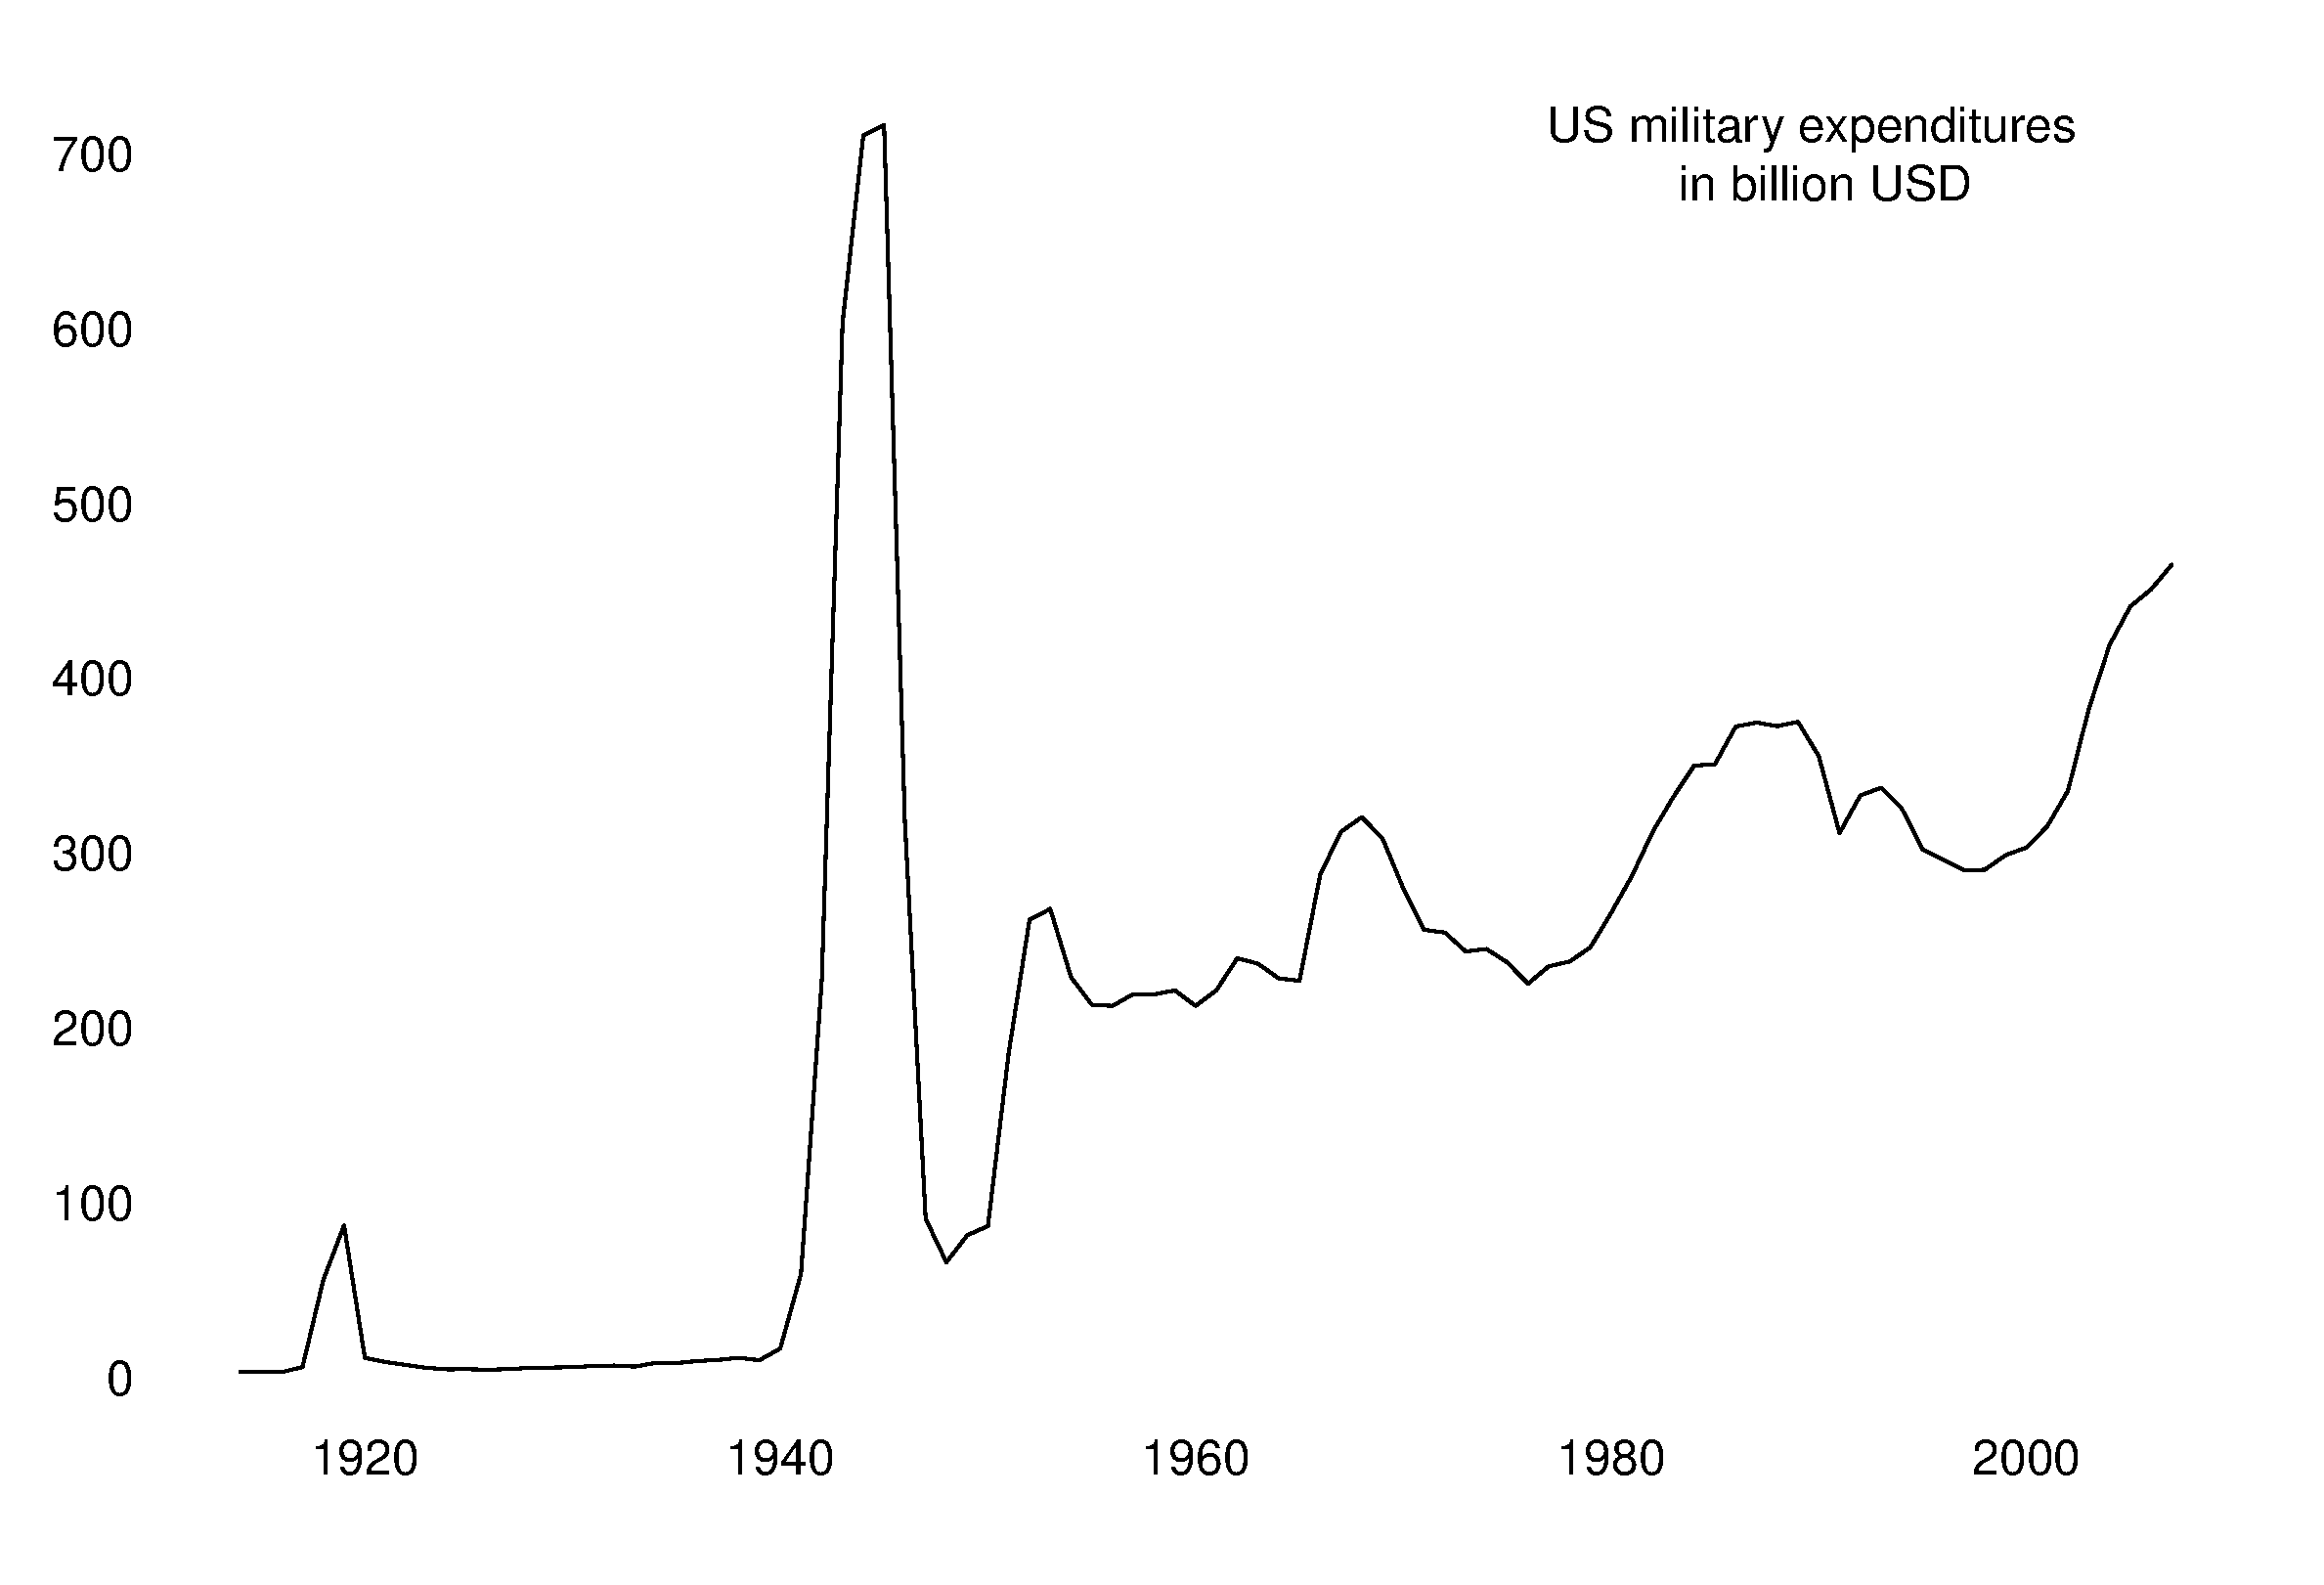
\includegraphics[scale=.3]{us_milexp.eps}
  \end{figure}
\end{frame}
%--------------------------------------

%--------------------------------------
\begin{frame}
  \begin{figure}
    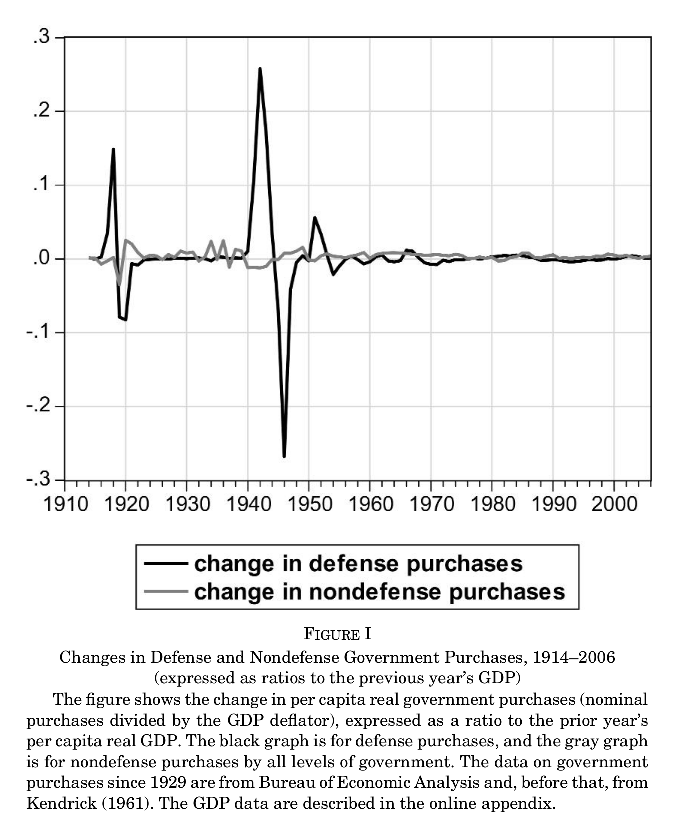
\includegraphics[scale=.5]{barro_redlick1.eps}
  \end{figure}
  Barro \& Redlick, 2011
\end{frame}
%--------------------------------------

%--------------------------------------
\begin{frame}
  \begin{figure}
    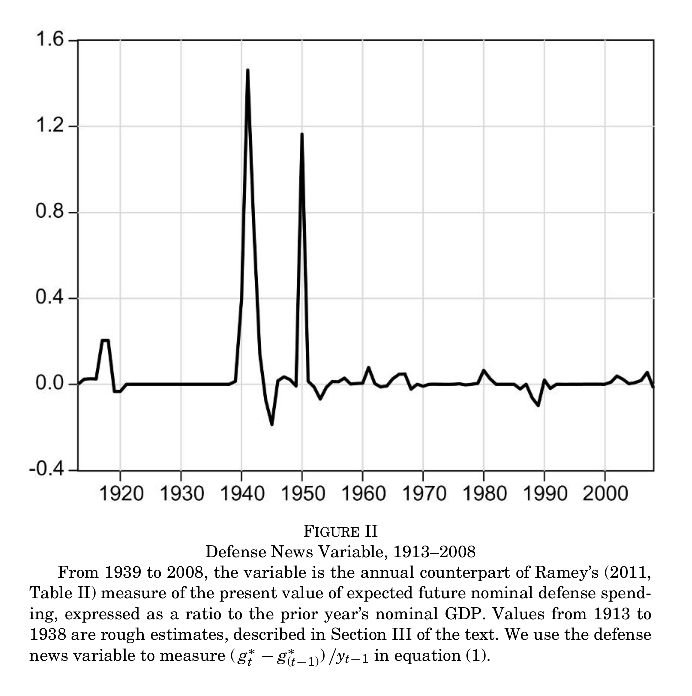
\includegraphics[scale=.5]{barro_redlick2.eps}
  \end{figure}
  Barro \& Redlick, 2011
\end{frame}
%--------------------------------------

%--------------------------------------
\begin{frame}
  \begin{figure}
    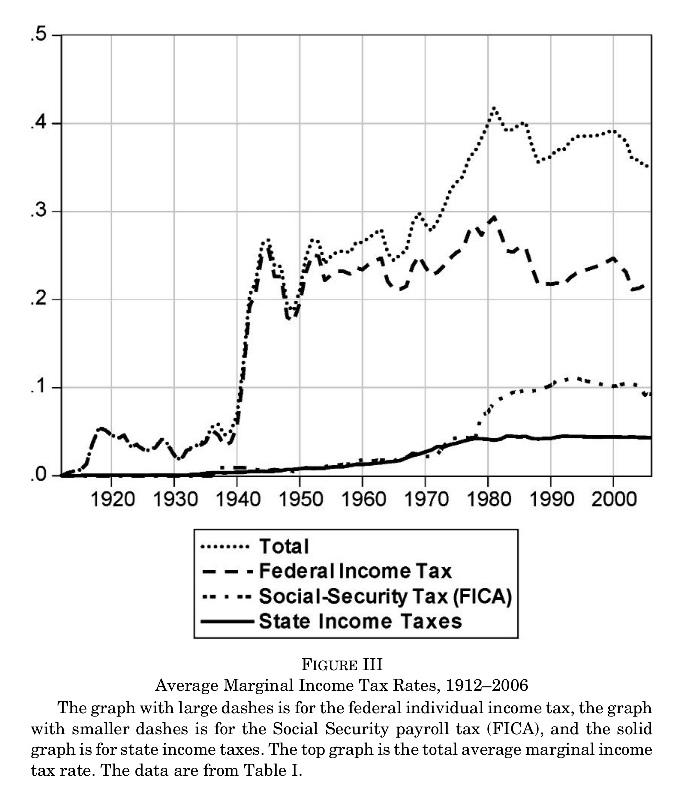
\includegraphics[scale=.5]{barro_redlick3.eps}
  \end{figure}
  Barro \& Redlick, 2011
\end{frame}
%--------------------------------------

%--------------------------------------
\begin{frame}
  \begin{figure}
    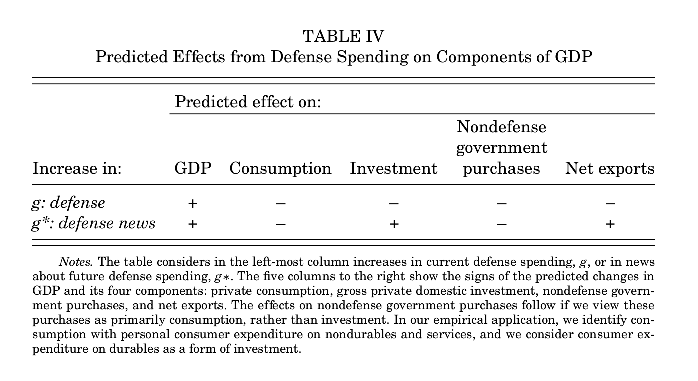
\includegraphics[scale=.6]{barro_redlick4.eps}
  \end{figure}
  Barro \& Redlick, 2011
\end{frame}
%--------------------------------------

%--------------------------------------
\begin{frame}
  Barro \& Redlick find that the estimated multiplier for temporary defence spending is
 \begin{enumerate}
   \item 0.4-0.5 contemporaneously (i.e. at year $t$)
   \item 0.6-0.7 over two years
 \end{enumerate}
 \medskip
 Magnitude of tax multiplier is $-$1.1
 \begin{itemize}
   \item Therefore the balanced budget-multiplier for defence spending is negative
   \item GDP will decline in response to higher defense spending and increased tax revenues
 \end{itemize}     
\end{frame}
%--------------------------------------

%--------------------------------------
\begin{frame}
 The non-neutrality of monetary policy is a contested area in macroeconomic research.  
 Nakamura \& Steinsson (2017) highlight three prominent pieces of evidence for non-neutrality
 \medskip
 \begin{enumerate}
   \item Poor Fed policy decisions prior to Great Depression, making things worse
   \item The Volcker disflation
   \item Break in volatility of US real exchange rate
 \end{enumerate} 
\end{frame}
%--------------------------------------

%--------------------------------------
\begin{frame}
  These pieces of evidence provide a useful insight into the preferred empirical methods
  \medskip  
  \begin{itemize}
    \item Two cases are exclusively based on historical events
    \item One is example of identification based on discontinuity
  \end{itemize}
  \medskip
  Not appearing in this list: VARs
\end{frame}
%--------------------------------------

%--------------------------------------
\begin{frame}
  In general there are four prevalent approaches in identifying the effect of monetary policy
  \begin{enumerate}
    \item Large shocks
    \item Narrative record to identify shocks
    \item Discontinuity-based identification    
    \item 'Controlling' for confounding factors, i.e. VAR methods
  \end{enumerate}
\end{frame}
%--------------------------------------

%--------------------------------------
\begin{frame}
 In empirical science the gold standard is of course the controlled experiment
 \medskip  
  \begin{itemize}
    \item Which for macro has become the holy grail as it is hard, if not impossible, to implement
  \end{itemize}
  \medskip
  Therefore, a fruitful approach is to look for large shocks or 'natural experiments'
  \begin{itemize}
    \item I.e. situations where policy changes are relatively large to potential confounding factors that cannot be accounted for
    \item These changes are few and far between 
  \end{itemize}
\end{frame}
%--------------------------------------

%--------------------------------------
\begin{frame}
  Friedman \& Schwartz (1963) is a good example of natural experiments: They argue that there were three policy actions by the Fed during the interbellum that were  
  \begin{enumerate}
    \item 'of major magnitude'
    \item 'cannot be regarded as necessary or inevitable economic consequences of contemporary changes in money income and prices'
  \end{enumerate}
  \medskip
  And
  \begin{quote}
    the results are so consistent and sharp as to leave little doubt about their interpretation
  \end{quote}
  \medskip
  The dates of these policy events are   
  \begin{itemize}
    \item January-June 1920
    \item October 1931
    \item July 1936 - January 1937
  \end{itemize}
\end{frame}
%--------------------------------------

%--------------------------------------
\begin{frame}
  \begin{figure}
    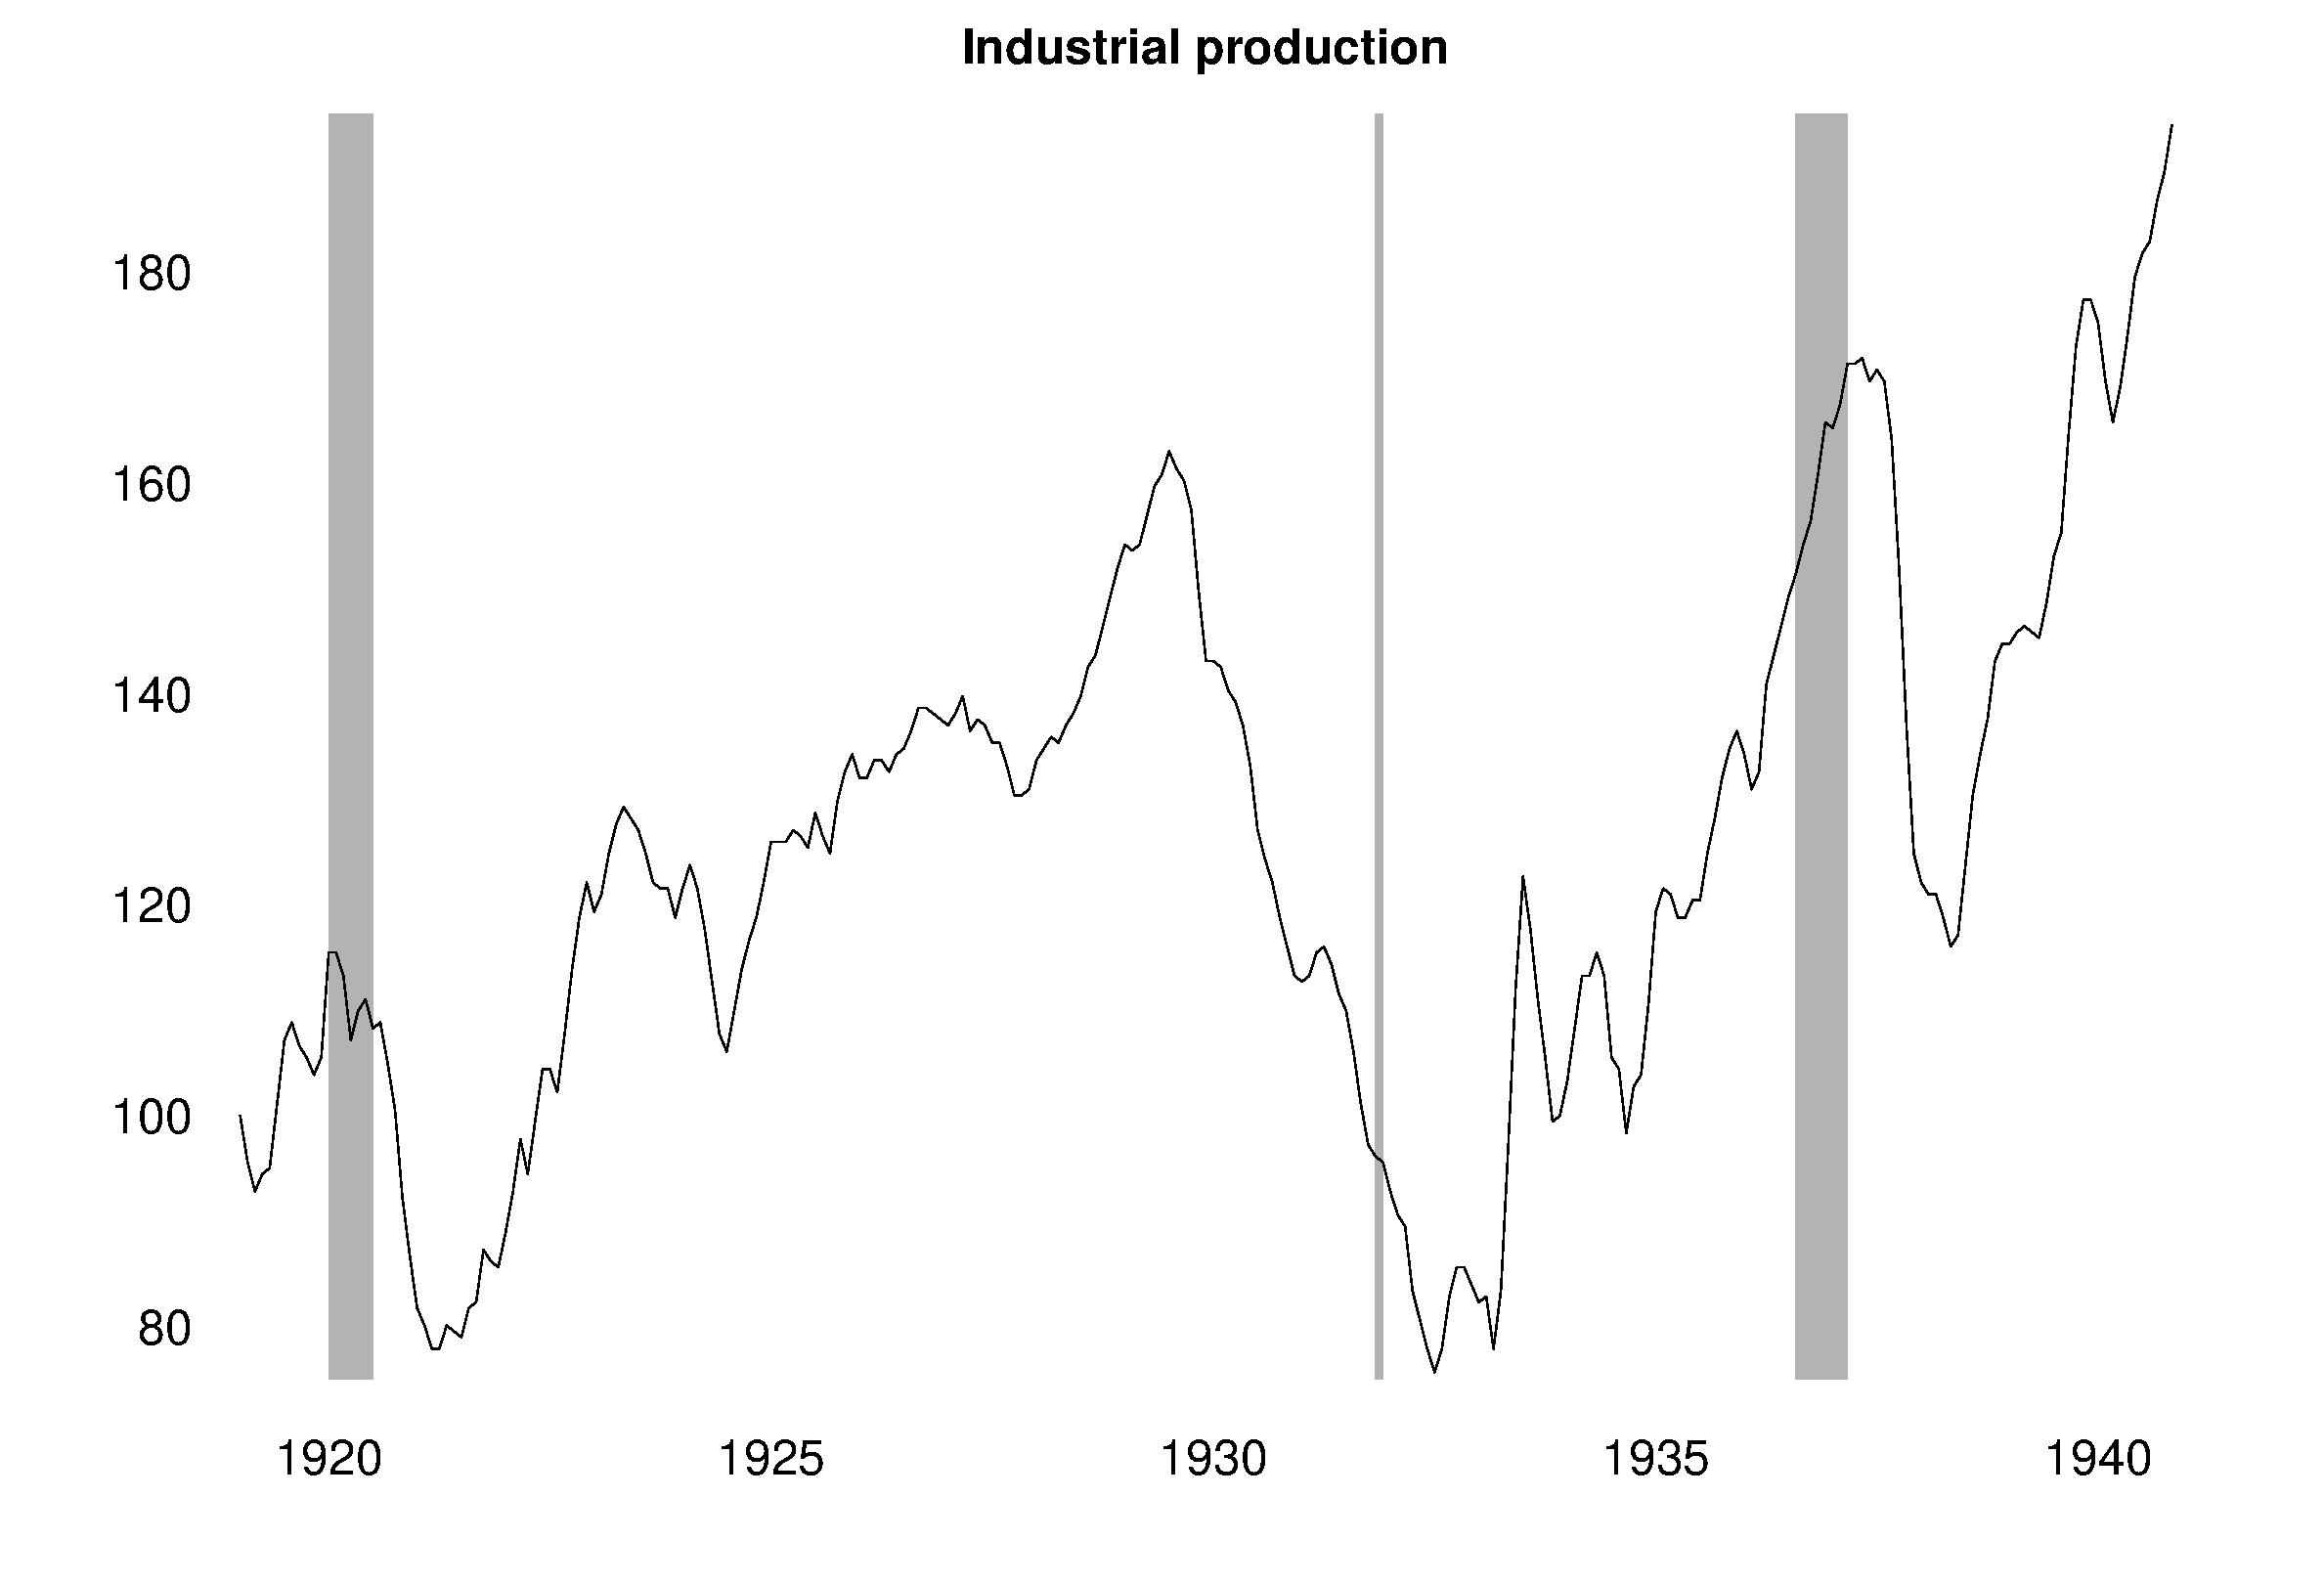
\includegraphics[scale=.3]{industrial_production.eps}
  \end{figure}
\end{frame}
%--------------------------------------

%--------------------------------------
\begin{frame}
 These policy mistakes, what were they exactly?
 Let's look at the decision made in October 1931
 \medskip
  \begin{itemize}
    \item Raise in discount rate from from 1.5\% to 3.5\%
    \item Response to potential speculative attacks on the US dollar following UK leaving the gold standard
  \end{itemize}  
\end{frame}
%--------------------------------------

%--------------------------------------
\begin{frame}
Fed tightened policy at a time that industrial production was decreasing rapidly; this might seem like clear monetary shock.
\medskip  
  \begin{itemize}
    \item Subsequent fall in industrial production, between October 1931- March 1933, not much different from preceding period
    \item Unclear how much of decrease can be attributed to policy shock
  \end{itemize}  
\end{frame}
%--------------------------------------

%--------------------------------------
\begin{frame}
 During the period July 1936-January 1937 two things happened
 \medskip
 \begin{enumerate}
   \item Fed announced doubling the reserve requirements (fully implemented May 1937)
   \item Treasury engaged in sterilisation of gold inflows
 \end{enumerate}
 \medskip
 Before this period there was a rapid rise in industrialisation but it was followed by a rapid decrease of 33\%
 \begin{itemize}
   \item 1937 recession might therefore be caused by slowdown in money creation due to policy actions
   \item Other factors at play though: tighter fiscal policy, constraints of gold standard
 \end{itemize}  
\end{frame}
%--------------------------------------


%--------------------------------------
\begin{frame}
  \begin{figure}
    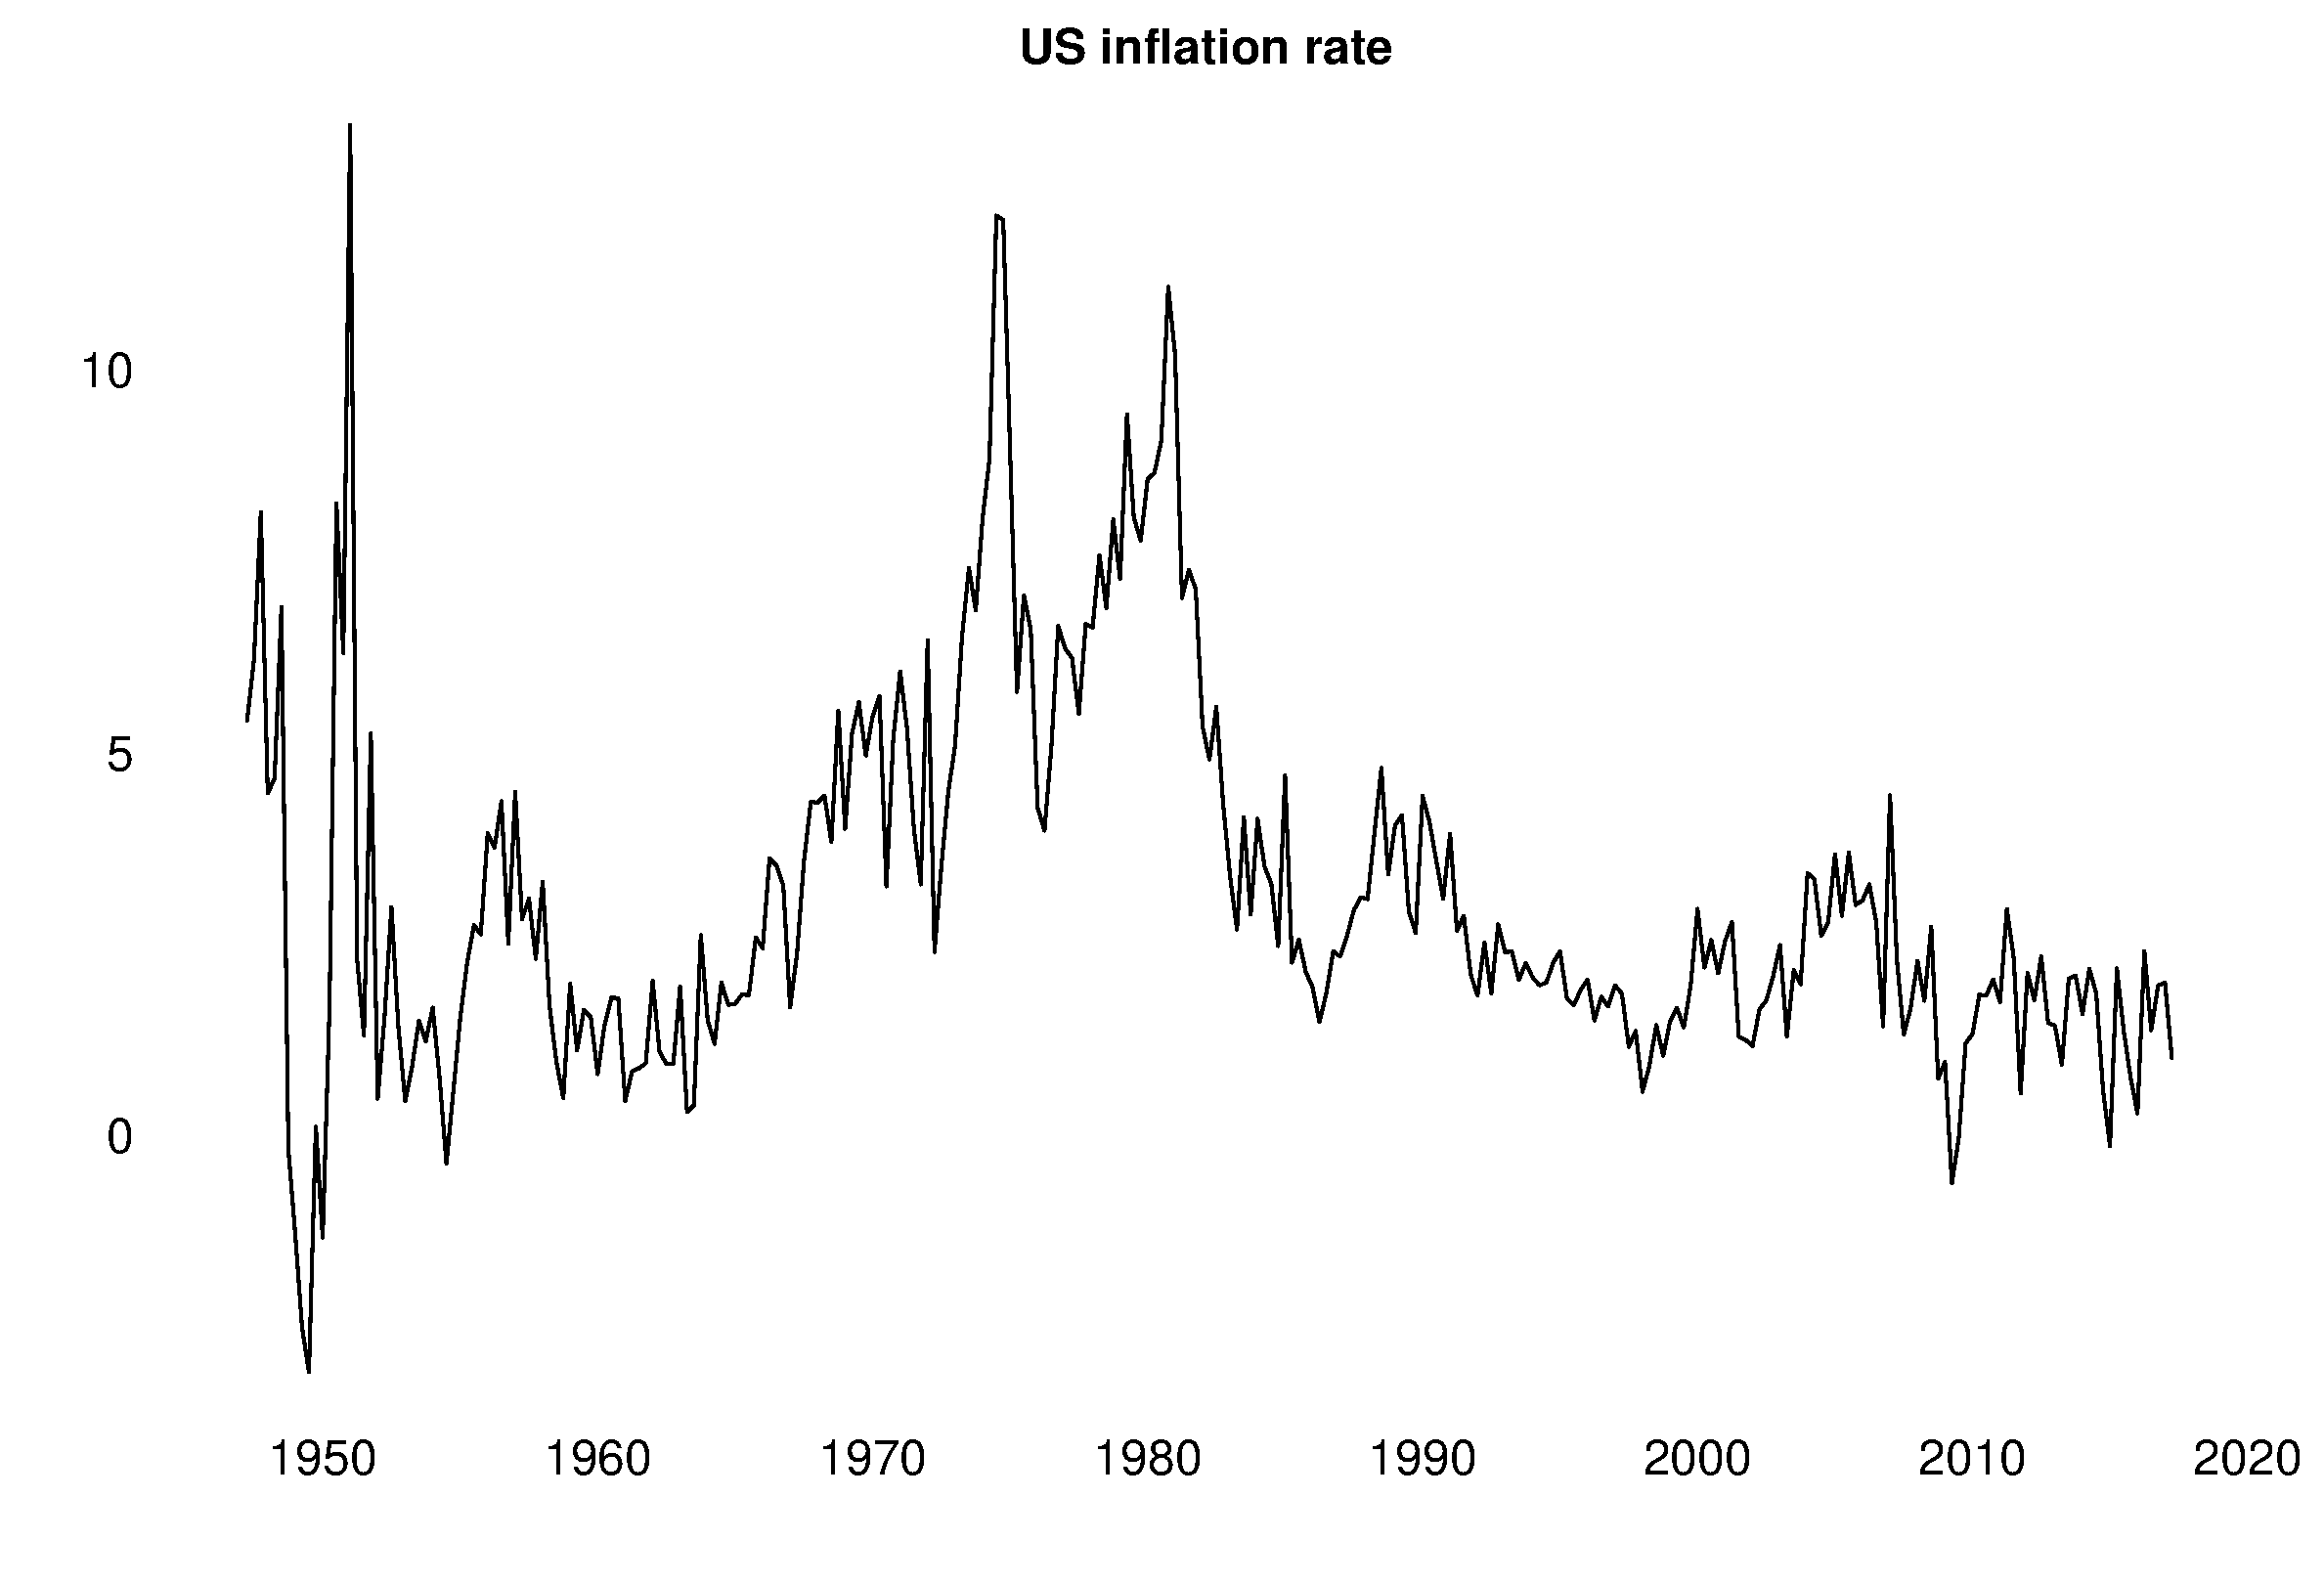
\includegraphics[scale=.29]{inflation.eps}
  \end{figure}
\end{frame}
%--------------------------------------


%--------------------------------------
\begin{frame}
  The Great Inflation of the 1970s followed a period of relatively stable and low inflation 
 \begin{itemize}
   \item Stable period after end of Korean War in 1953, inflation started to rise in the 1960s
   \item During 1970s inflation was high and volatile, often in double digits
 \end{itemize}
 \medskip
 During this period monetary policy was characterised by 'stop-go' 
 \begin{itemize}
   \item Tight when the public was concerned about inflation, loose when public was concerned about unemployment
 \end{itemize}
 \medskip
 Volcker  disflation followed after Volcker was appointed as chairman of the Federal Reserve Board in August 1979
 \begin{itemize}
   \item Volcker broke with modus operandi and targeted deliberate disinflation  
 \end{itemize}  
\end{frame}
%--------------------------------------

%--------------------------------------
\begin{frame}
  \begin{figure}
    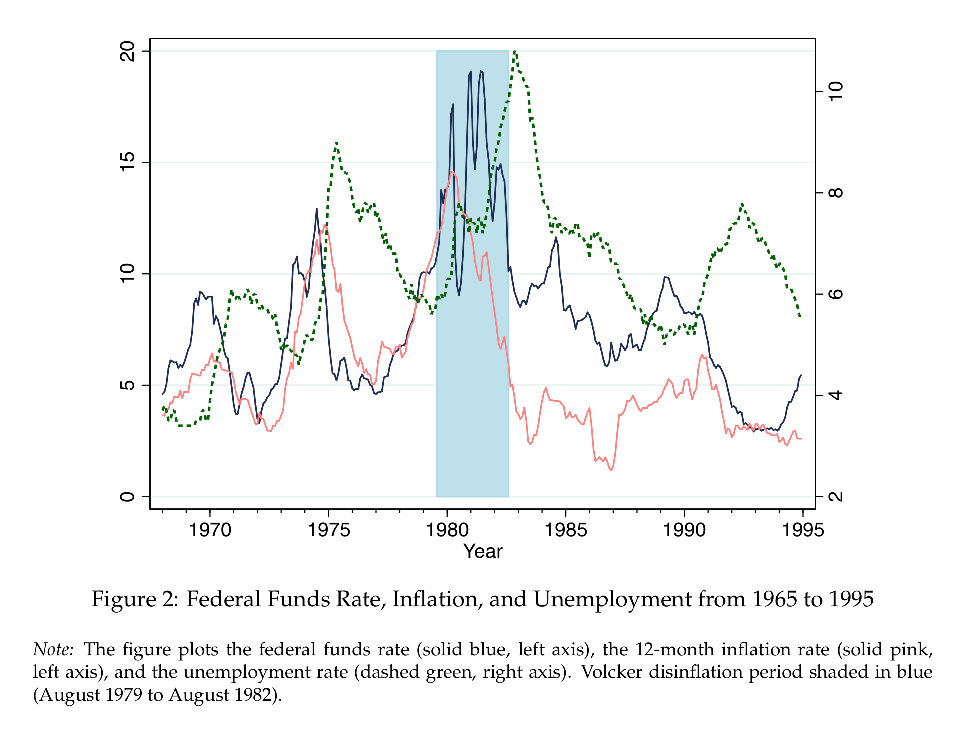
\includegraphics[scale=.6]{nakamura_steinsson.eps}
  \end{figure}
  Nakamura \& Steinsson (2017)
\end{frame}
%--------------------------------------

%--------------------------------------
\begin{frame}
  \begin{figure}
    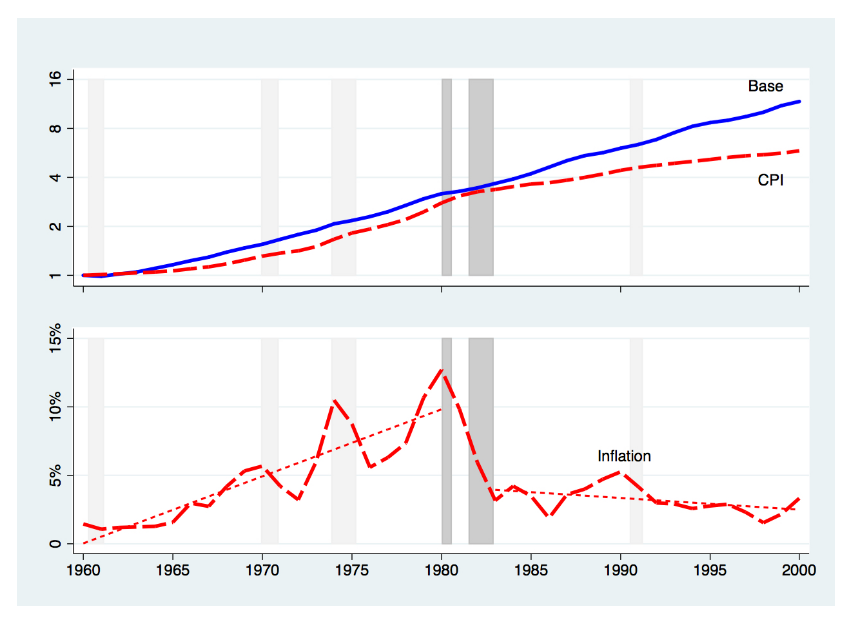
\includegraphics[scale=.7]{romer.eps}
  \end{figure}
  Romer (2016)
\end{frame}
%--------------------------------------

%--------------------------------------
\begin{frame}
  During the 1980s output seemed indeed to respond to monetary policy, but there are other factors
  \begin{enumerate}
    \item Oil shocks in 1979/1980
    \item Credit controls in 1980
    \item Tax cuts in 1981-82
  \end{enumerate}
  \medskip
  Volcker episode is consistent with non-neutrality of monetary policy, but not concerning idea that policy affects output with long and variable lags.
  \begin{itemize}
    \item Output reacted largely synchronised with Fed actions
  \end{itemize}  
\end{frame}
%--------------------------------------
%--------------------------------------
\begin{frame}
  \begin{figure}
    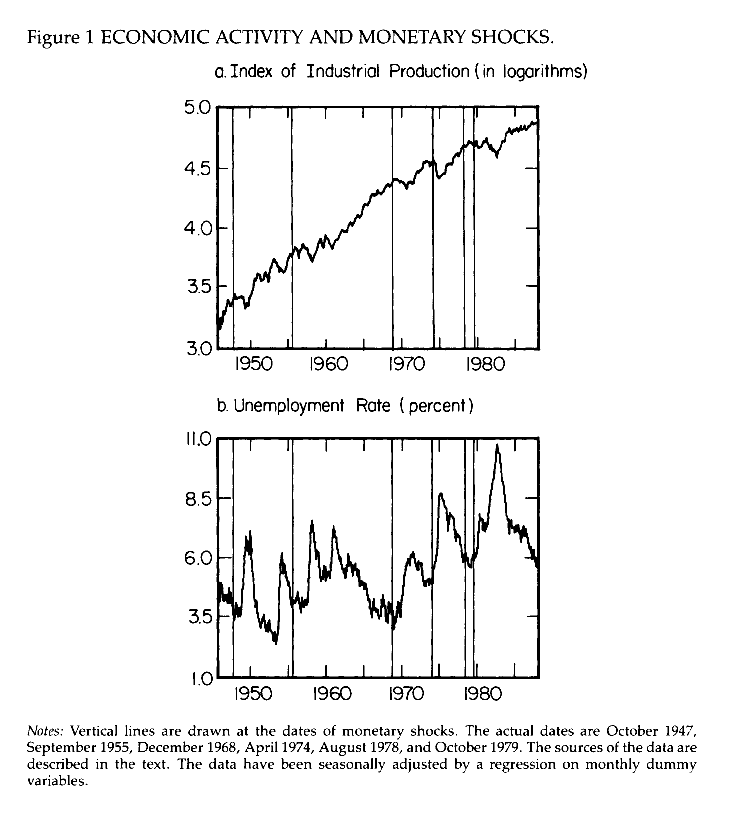
\includegraphics[scale=.6]{romer_romer.eps}
  \end{figure}
  Romer \& Romer (1989)
\end{frame}
%--------------------------------------

%--------------------------------------
\begin{frame}
  Romer \& Romer (1989) use the narrative record to search for natural experiments
  \begin{itemize}
    \item Based on Fed records, identifying attempts to create recession to reduce inflation
    \item There are 6 Romer-Romer dates
    \item Find that shift to anti-inflationary policy led to increase in unemployment
  \end{itemize}
  \medskip
  Their work is based on the paper by Friedmand \& Schwartz (1963) earlier mentioned
  \begin{itemize}
    \item Indeed the title is 'Does monetary policy matter? A new test in the spirit of Friedman and Schwartz'
  \end{itemize}    
\end{frame}
%--------------------------------------

%--------------------------------------
\begin{frame}
  There are a number of shortcomings associated with this approach  
  \begin{enumerate}
    \item Unclear how narrative record is selected; risk of reverse-engineering 
    \item Few data points; some other factor might be correlated with monetary shock, e.g. oil shocks
    \item Shocks are endogenous because they might be predictable; hard to establish though
  \end{enumerate}
\end{frame}
%--------------------------------------

%--------------------------------------
\begin{frame}
  Finally there is the approach using \textbf{discontinuity-based} identification
  \medskip
  \begin{itemize}
    \item Quasi-experimental based on using some event as an intervention allowing for comparison of pre- and post situation 
    \item The identifying assumption made is that other factors affecting the exchange rate do not change discontinuously
  \end{itemize}
  \medskip
  Seminal paper on monetary policy is Mussa (1986) using a change in exchange rate regime
\end{frame}
%--------------------------------------

%--------------------------------------
\begin{frame}
  \begin{figure}
    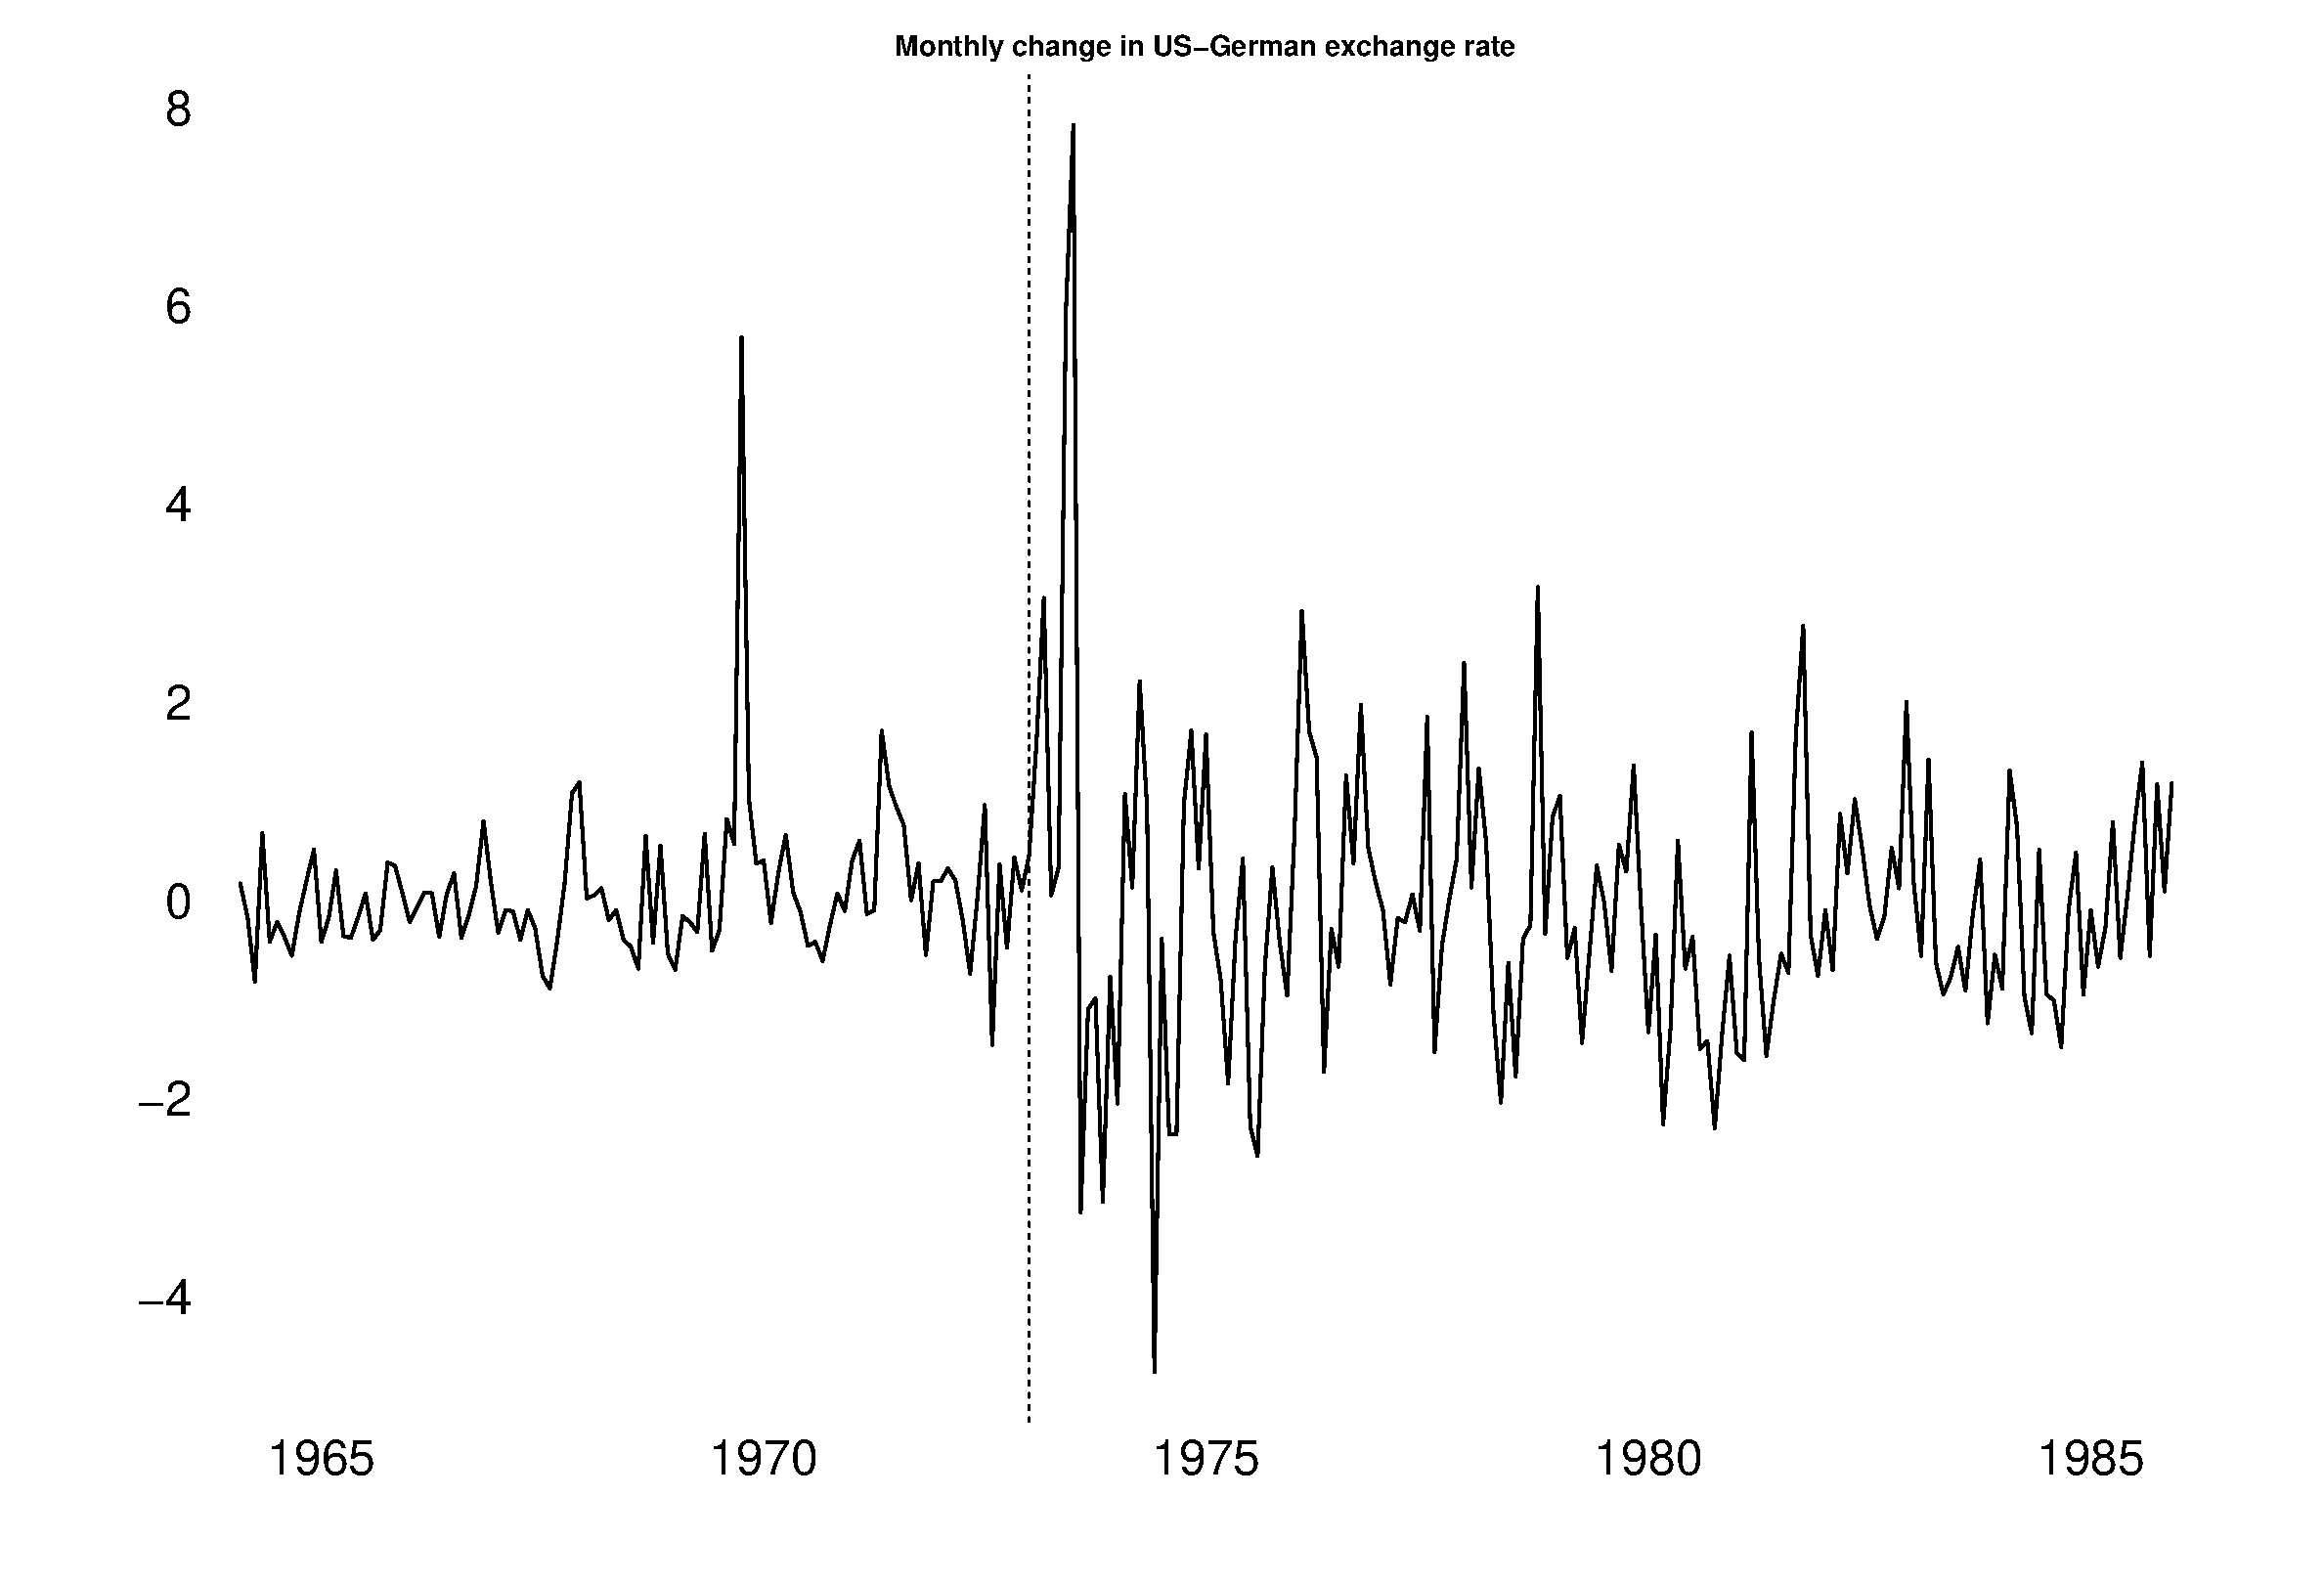
\includegraphics[scale=.3]{exchange_rate.eps}
  \end{figure}  
\end{frame}
%--------------------------------------

%--------------------------------------
\begin{frame}
  Under Bretton-Woods system exchange rates were fixed
  \begin{itemize}
    \item Made US dollar reserve currency, other currencies were to be maintained within 1\% band
    \item System broke down in February 1973; Japan and EEC countries let their currency float
    \item Breakdown caused large increase in volatility of US exchange rate
  \end{itemize}
  \medskip  
\end{frame}
%--------------------------------------


%--------------------------------------
\begin{frame}
 Mussa (1986) associated the breakdown of the system, the result of change in monetary policy, with increase in real exchange rate
  \begin{itemize}
    \item Note that switching exchange rate regime from fixed to flexible is strictly monetary action
    \item If monetary policy is neutral, this change should have no impact on real variables such as real exchange rate
  \end{itemize}
  \medskip
  Instead, Mussa found a more than fourfold increase in the standard deviation  
\end{frame}
%--------------------------------------



%--------------------------------------
\end{document}
